\chapter{Alquenos y alquinos: adiciones electrófilas}\label{ch:b1:electrophilic-additions}

Agítese un alqueno con agua de bromo naranja y el color desaparece en
segundos: es la prueba más antigua de un enlace doble carbono--carbono.
Detrás hay un mecanismo. Los electrones $\pi$ del enlace doble, retenidos
con menos fuerza que los electrones $\sigma$ y expuestos por encima y por
debajo del plano de la molécula, atacan un reactivo pobre en electrones;
el catión formado captura después un \omterm{def:b1:electronic-effects:nucleophile}{nucleófilo}. Las mismas dos etapas
adicionan a los alquenos los haluros de hidrógeno, el agua y los
halógenos, deciden qué carbono recibe cada parte del reactivo y fijan la
estereoquímica del producto. Este capítulo las desarrolla, con la regla
que un químico del siglo XIX extrajo de la observación y el \omterm{def:b1:electronic-effects:intermediates}{carbocatión}
que la explica.

\begin{recall}
Los \omterm{def:b1:electronic-effects:intermediates}{carbocationes}, su estabilidad y las \omterm{def:b1:electronic-effects:curly-arrow}{flechas curvas}
(\cref{ch:b1:electronic-effects}); el postulado de Hammond
(\cref{prop:b1:elementary-steps:hammond}); los descriptores $Z$/$E$,
\cip{R}/\cip{S}, los \omterm{def:b1:stereochemistry-in-depth:enantiomers}{compuestos meso} y las \omterm{def:b1:stereochemistry-in-depth:enantiomers}{mezclas racémicas}
(\cref{ch:b1:stereochemistry-in-depth}). El volumen escolar (año 12)
enumeró las adiciones de los alquenos sin sus mecanismos.
\end{recall}

\section{El enlace \texorpdfstring{$\pi$}{pi} como nucleófilo}

\begin{definition}[Adición electrófila]\label{def:b1:electrophilic-additions:electrophilic-addition}
Una \emph{adición electrófila}\index{adicion electrofila@adición electrófila} a un
enlace múltiple es una adición cuya primera etapa es el ataque de los
electrones $\pi$ sobre un \omterm{def:b1:electronic-effects:nucleophile}{electrófilo} E: se forma un catión, que captura
después un \omterm{def:b1:electronic-effects:nucleophile}{nucleófilo} Nu, de modo que E y Nu terminan en los dos carbonos
del antiguo enlace doble.
\end{definition}

El enlace $\pi$ es el más débil de los dos enlaces de C=C
(\cref{ch:b1:lewis-resonance-vsepr}), y sus electrones se sitúan lejos de
los núcleos, por encima y por debajo del plano: los alquenos son
\omterm{def:b1:electronic-effects:nucleophile}{nucleófilos}, y reaccionan con los ácidos, los halógenos y otros
\omterm{def:b1:electronic-effects:nucleophile}{electrófilos} que dejan intactos los alcanos saturados.

\section{Adición de haluros de hidrógeno: la regla de Markovnikov}

\begin{omfigure}
\setchemfig{atom sep=2.1em}
\schemestart
\chemfig{H_3C-[:30]@{c2}CH=[@{pi},,,,]@{c1}CH_2}
\+
\chemfig{@{h}H-[@{hb}]@{br}Br}
\arrow{->}
\chemfig{H_3C-[:30]CH^{+}-[:-30]CH_3}
\+
\chemfig{Br^{-}}
\arrow{->}
\chemfig{H_3C-[:30]CH(-[2]Br)-[:-30]CH_3}
\schemestop
\chemmove{\draw[->, thick, shorten <=2pt, shorten >=2pt](pi) .. controls +(90:7mm) and +(110:7mm) .. (h);
          \draw[->, thick, shorten <=2pt, shorten >=2pt](hb) .. controls +(-90:5mm) and +(-90:5mm) .. (br);}

{\small Adición de bromuro de hidrógeno al propeno. El par $\pi$ toma el
protón y lo une al carbono terminal, lo que da el \omterm{def:b1:electronic-effects:intermediates}{carbocatión} secundario;
el ion bromuro se adiciona a él: 2-bromopropano.}
\end{omfigure}

\begin{proposition}[Regla de Markovnikov]\label{prop:b1:electrophilic-additions:markovnikov}
En la adición de HX a un alqueno asimétrico, el hidrógeno se une al
carbono del enlace doble que ya lleva más hidrógenos (\emph{regla de
Markovnikov}\index{regla de Markovnikov}). En forma moderna: el
\omterm{def:b1:electronic-effects:nucleophile}{electrófilo} se adiciona de modo que dé el \omterm{def:b1:electronic-effects:intermediates}{carbocatión} más estable.
\end{proposition}

\begin{proof}
La transferencia del protón es la \omterm{def:b1:elementary-steps:rds}{etapa determinante de la velocidad},
endotérmica, y termina en un \omterm{def:b1:electronic-effects:intermediates}{carbocatión}. Según el postulado de Hammond
(\cref{prop:b1:elementary-steps:hammond}), su \omterm{def:b1:elementary-steps:energy-profile}{estado de transición} se
parece al \omterm{def:b1:electronic-effects:intermediates}{carbocatión}, de modo que el camino hacia el \omterm{def:b1:electronic-effects:intermediates}{carbocatión} más
estable tiene la barrera más baja y es mucho más rápido. Poner el protón
en el carbono con más hidrógenos deja la carga en el carbono con más
grupos alquilo, el catión más estable
(\cref{prop:b1:electronic-effects:carbocation-order}).
\end{proof}

\begin{omfigure}
\begin{tikzpicture}
\begin{axis}[
  width=0.78\linewidth, height=5.0cm, xmin=0, xmax=10, ymin=-45, ymax=125,
  axis x line=bottom, axis y line=left, xlabel={coordenada de reacción},
  ylabel={energía}, xtick=\empty, ytick=\empty, label style={font=\small},
  legend style={font=\scriptsize, draw=none, at={(0.5,-0.30)}, anchor=north}, legend columns=2]
\addplot[omThm, thick, dashed] table[x=x, y=E] {figdata/out/bachelor-1-energy-profiles-primary.dat};
\addplot[omDef, very thick] table[x=x, y=E] {figdata/out/bachelor-1-energy-profiles-secondary.dat};
\legend{vía el catión primario, vía el catión secundario}
\node[font=\scriptsize, anchor=south] at (axis cs:5,103) {\ce{CH3CH2CH2+}};
\draw[omThm, densely dotted] (axis cs:5,103) -- (axis cs:5,87);
\node[font=\scriptsize, anchor=north] at (axis cs:5,43) {\ce{CH3CH+CH3}};
\node[font=\scriptsize, anchor=north west] at (axis cs:0.1,-3) {propeno + HBr};
\end{axis}
\end{tikzpicture}

{\small \omterm{def:b1:elementary-steps:energy-profile}{Perfiles de energía} esquemáticos de las dos adiciones posibles de
HBr al propeno. El \omterm{def:b1:electronic-effects:intermediates}{carbocatión} secundario, más estable, está más bajo y,
según el postulado de Hammond, también lo está el \omterm{def:b1:elementary-steps:energy-profile}{estado de transición}
que conduce a él: el producto de Markovnikov se forma mucho más deprisa.}
\end{omfigure}

\begin{definition}[Transposición de carbocationes]\label{def:b1:electrophilic-additions:rearrangement}
Una \emph{transposición de carbocationes}\index{transposicion de carbocationes@transposición de carbocationes} es la
migración, dentro de un \omterm{def:b1:electronic-effects:intermediates}{carbocatión}, de un átomo de hidrógeno o de un
grupo alquilo con su par de enlace al carbono catiónico vecino, que da un
\omterm{def:b1:electronic-effects:intermediates}{carbocatión} más estable (una migración 1,2).
\end{definition}

\begin{example}[Una migración de metilo]\label{ex:b1:electrophilic-additions:shift}
El 3,3-dimetilbut-1-eno y el cloruro de hidrógeno dan un \omterm{def:b1:electronic-effects:intermediates}{carbocatión}
secundario contiguo a un carbono cuaternario; un grupo metilo se desplaza
con su par y forma un catión terciario. El producto principal es el
2-cloro-2,3-dimetilbutano, cuyo esqueleto difiere del del alqueno; el
3-cloro-2,2-dimetilbutano es minoritario.
\end{example}

\begin{omfigure}
\setchemfig{atom sep=2em}
\schemestart
\chemfig{C(-[2]CH_3)(-[6]CH_3)(-[4]H_3C)-CH^{+}-CH_3}
\arrow{->[migr. 1,2]}[,1.5]
\chemfig{C^{+}(-[2]CH_3)(-[4]H_3C)-CH(-[6]CH_3)-CH_3}
\arrow{->[\ce{Cl-}]}
\chemfig{C(-[2]CH_3)(-[6]Cl)(-[4]H_3C)-CH(-[6]CH_3)-CH_3}
\schemestop
\par\vspace{6pt}

{\small Transposición del catión 3,3-dimetilbutan-2-ilo: un grupo metilo
migra al carbono catiónico y convierte un catión secundario en uno
terciario, que el cloruro captura.}
\end{omfigure}

\section{Adición de agua}

\begin{definition}[Hidratación de un alqueno]\label{def:b1:electrophilic-additions:hydration}
La \emph{hidratación}\index{hidratacion@hidratación} de un alqueno es la adición de
agua, catalizada por un \omterm{def:b1:predominant-reaction:strong-acid}{ácido fuerte}, que da un alcohol: la reacción
inversa de la \omterm{def:b1:alcohol-activation:dehydration}{deshidratación} del \cref{ch:b1:alcohol-activation}.
\end{definition}

El mecanismo es el de HX con el agua como \omterm{def:b1:electronic-effects:nucleophile}{nucleófilo}: protonación
(Markovnikov), captura del \omterm{def:b1:electronic-effects:intermediates}{carbocatión} por el agua y pérdida de un protón
del ion oxonio. El propeno da propan-2-ol; el 2-metilpropeno,
2-metilpropan-2-ol. La \omterm{def:b1:electrophilic-additions:hydration}{hidratación} y la \omterm{def:b1:alcohol-activation:dehydration}{deshidratación} son el mismo
equilibrio, \ce{C3H6 + H2O <=> C3H8O}; el ácido acuoso diluido y la
temperatura baja favorecen el alcohol, y el ácido concentrado, el calor y
la eliminación del alqueno favorecen el alqueno
(\cref{ch:b1:extent-q-and-k}).

\section{Adición de halógenos: iones halonio y adición anti}

\begin{definition}[Ion halonio, adición anti y sin]\label{def:b1:electrophilic-additions:halonium}
En la adición de \ce{Br2} o de \ce{Cl2}, el par $\pi$ ataca a un átomo de
halógeno mientras un \omterm{def:b1:lewis-resonance-vsepr:lewis}{par no enlazante} de ese átomo se une al segundo
carbono: se forma un \emph{ion halonio}\index{ion halonio} cíclico de tres
miembros, y el otro halógeno sale como haluro. Una adición en la que los
dos nuevos grupos terminan en caras opuestas del antiguo enlace doble es
una \emph{adición anti}\index{adicion anti@adición anti}; en la misma cara, una \emph{adición
sin}\index{adicion sin@adición sin}.
\end{definition}

\begin{proposition}[La adición de halógenos es anti]\label{prop:b1:electrophilic-additions:anti-addition}
La adición de bromo a un alqueno es una \omterm{def:b1:electrophilic-additions:halonium}{adición anti}: el
\cip{E}-but-2-eno da meso-2,3-dibromobutano, y el \cip{Z}-but-2-eno da la
\omterm{def:b1:stereochemistry-in-depth:enantiomers}{mezcla racémica} de \cip{2R,3R}- y \cip{2S,3S}-2,3-dibromobutano.
\end{proposition}

\begin{proof}
El ion bromonio forma un puente sobre una cara del antiguo enlace doble;
el bromuro solo puede atacar un carbono por la otra cara, y abre el
anillo como en una SN2, con inversión en ese carbono. Los dos bromos
terminan en caras opuestas. Para el \cip{E}-but-2-eno, el ataque a
cualquiera de los dos carbonos da el mismo producto, en el que los dos
\omterm{def:b1:stereochemistry-in-depth:stereocentre}{centros estereogénicos} son imagen especular el uno del otro:
\cip{2R,3S}, meso. Para el \cip{Z}-but-2-eno, el ataque a un carbono da
\cip{2R,3R}, y al otro, \cip{2S,3S}, con igual probabilidad: una \omterm{def:b1:stereochemistry-in-depth:enantiomers}{mezcla
racémica}. La demostración mediante dibujos es el
\cref{exo:b1:electrophilic-additions:10}.
\end{proof}

\begin{omfigure}
\begin{tikzpicture}[font=\small, >={Stealth}]
  % bromonium ion from (E)-but-2-ene
  \coordinate (a) at (0,0); \coordinate (b) at (1.4,0);
  \draw[thick] (a) -- (b);
  \node[circle, fill=white, inner sep=1pt] (br) at (0.7,1.0) {\ce{Br+}};
  \draw[thick] (a) -- (br.south west) (b) -- (br.south east);
  \draw[thick] (a) -- ++(-0.8,0.35) node[left] {H};
  \draw[thick] (a) -- ++(-0.6,-0.6) node[below left] {\ce{CH3}};
  \draw[thick] (b) -- ++(0.8,0.35) node[right] {\ce{CH3}};
  \draw[thick] (b) -- ++(0.6,-0.6) node[below right] {H};
  \node (bm) at (0.7,-1.6) {\ce{Br-}};
  \draw[->, thick, omThm] (bm) to[bend left=25] (0.12,-0.12);
  \node[align=center] at (0.7,-2.4) {ataque por la cara opuesta al puente};
  \draw[->, thick] (3.3,0) -- (4.4,0);
  \node[align=center] at (6.2,0) {\chemfig{C(-[:150]H_3C)(<[:210]H)(<:[2]Br)-C(<:[:30]H)(-[:-30]CH_3)(<[6]Br)}};
  \node at (6.2,-1.8) {producto anti: meso-2,3-dibromobutano};
\end{tikzpicture}

{\small El ion bromonio formado a partir del \cip{E}-but-2-eno, y su
apertura por el bromuro desde la cara opuesta (\omterm{def:b1:electrophilic-additions:halonium}{adición anti}). El
producto tiene dos \omterm{def:b1:stereochemistry-in-depth:stereocentre}{centros estereogénicos} de descriptores opuestos y un
plano de simetría interno en una \omterm{def:b1:stereochemistry-in-depth:isomers}{conformación} adecuada: el \omterm{def:b1:stereochemistry-in-depth:enantiomers}{compuesto
meso}, \cip{2R,3S}.}
\end{omfigure}

\begin{inthelab}[El agua de bromo]
El bromo es un líquido denso, volátil, muy tóxico y corrosivo. La prueba
de insaturación usa agua de bromo diluida (o una disolución comercial de
un \omterm{def:b1:complexation:complex}{complejo} de bromo) en una vitrina de gases, unas gotas cada vez; la
desaparición del color naranja indica una adición. En agua, el ion
bromonio también es capturado por el agua, y se forma una bromohidrina
junto al dibromuro.
\end{inthelab}

\section{Alquinos: adiciones y acetiluros}

Los alquinos adicionan HX y \ce{X2} dos veces, cada etapa como en los
alquenos (Markovnikov para HX). Su \omterm{def:b1:electrophilic-additions:hydration}{hidratación}, catalizada por un ácido y
una sal de mercurio(II), no da el alcohol insaturado esperado sino una
cetona: un enol se transforma de inmediato en el compuesto carbonílico,
un proceso que se estudia en el volumen del segundo año.

\begin{definition}[Alquino terminal, acetiluro]\label{def:b1:electrophilic-additions:acetylide}
Un \emph{alquino terminal}\index{alquino terminal} \ce{R-C#C-H} tiene su
enlace triple al final de la cadena. Una \omterm{def:b1:predominant-reaction:strong-acid}{base fuerte} (la amida de sodio)
le arranca el hidrógeno y da el \emph{ion acetiluro}\index{ion acetiluro}
\ce{R-C#C-}, un buen \omterm{def:b1:electronic-effects:nucleophile}{nucleófilo} carbonado.
\end{definition}

\begin{proposition}[Acidez de los alquinos terminales]\label{prop:b1:electrophilic-additions:acetylide-acidity}
El enlace C--H de un \omterm{def:b1:electrophilic-additions:acetylide}{alquino terminal} es mucho más ácido que los de los
alquenos y los alcanos, aunque todavía mucho menos ácido que el agua: los
acetiluros se forman con iones amiduro, no con hidróxido, y el agua los
destruye.
\end{proposition}

\begin{proof}
En el \omterm{def:b1:electrophilic-additions:acetylide}{ion acetiluro}, el \omterm{def:b1:lewis-resonance-vsepr:lewis}{par no enlazante} ocupa un orbital con un
cincuenta por ciento de carácter \textit{s} (carbono \textit{sp}),
retenido más cerca del núcleo que los orbitales de los \omterm{def:b1:electronic-effects:intermediates}{carbaniones}
\textit{sp}$^2$ o \textit{sp}$^3$: es más estable, y su ácido conjugado,
más fuerte. Sigue siendo una base mucho más fuerte que el hidróxido, de
modo que el agua lo protona.
\end{proof}

Un acetiluro ataca un haloalcano primario por SN2 (un nuevo enlace C--C,
\ce{R-C#C-} + $\mathrm{R'Br}$) o se adiciona a un carbonilo como un
\omterm{def:b1:organomagnesium:organometallic}{reactivo de Grignard}: otra forma de construir esqueletos carbonados.

\begin{method}[Predecir una adición]\label{met:b1:electrophilic-additions:predict-addition}
\begin{enumerate}
  \item Se identifican el \omterm{def:b1:electronic-effects:nucleophile}{electrófilo} (\ce{H+}, \ce{Br2}) y el \omterm{def:b1:electronic-effects:nucleophile}{nucleófilo}
        que vendrá después (\ce{X-}, el agua, el haluro).
  \item Para \ce{H+}: se une al carbono que da el \omterm{def:b1:electronic-effects:intermediates}{carbocatión} más estable
        (Markovnikov); se comprueba si es posible una migración 1,2.
  \item Para \ce{X2}: se forma el puente del \omterm{def:b1:electrophilic-additions:halonium}{ion halonio} y se abre desde la
        cara opuesta (anti); se dibujan los dos ataques posibles y se
        comparan los productos (meso o racémico).
  \item En presencia de agua, se espera también el alcohol (o la
        halohidrina).
\end{enumerate}
\end{method}

\begin{history}[Vladímir Markóvnikov]
\begin{minipage}[t]{0.2\linewidth}\vspace{0pt}
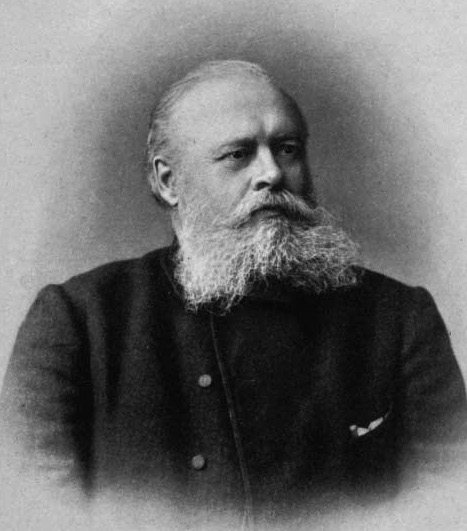
\includegraphics[width=\linewidth]{images/book2/markovnikov.jpg}
\end{minipage}\hfill
\begin{minipage}[t]{0.76\linewidth}\vspace{0pt}
Vladímir Markóvnikov enunció su regla en el siglo XIX, a partir de los
productos que él y otros observaban, mucho antes de que existieran los
\omterm{def:b1:electronic-effects:intermediates}{carbocationes} o las \omterm{def:b1:electronic-effects:curly-arrow}{flechas curvas}: una regularidad de la naturaleza,
escrita antes de poder explicarse. Su enunciado moderno, a través de la
estabilidad de los \omterm{def:b1:electronic-effects:intermediates}{carbocationes}, muestra lo que un mecanismo añade a
una regla empírica: dice cuándo debería fallar la regla. (Retrato
procedente de una nota necrológica publicada en 1905, dominio público,
Wikimedia Commons.)
\end{minipage}
\end{history}

\section{Ejercicios}

\begin{exercise}[$\star$]\label{exo:b1:electrophilic-additions:1}
Dese el producto principal de: propeno + HCl; 2-metilpropeno + HBr;
1-metilciclohexeno + HBr; but-2-ino + un equivalente de HCl.
\end{exercise}

\begin{exercise}[$\star$]\label{exo:b1:electrophilic-additions:2}
Escríbanse los productos del bromo con el eteno, el ciclohexeno y el
propeno. Nómbrense.
\end{exercise}

\begin{exercise}[$\star$]\label{exo:b1:electrophilic-additions:3}
¿Qué alcohol da la \omterm{def:b1:electrophilic-additions:hydration}{hidratación} catalizada por ácido de cada alqueno:
propeno, 2-metilpropeno, metilenciclohexano?
\end{exercise}

\begin{exercise}[$\star$]\label{exo:b1:electrophilic-additions:4}
¿Cuáles de estos compuestos reaccionan con la amida de sodio: propino,
but-2-ino, propeno, etanol? Escríbanse las reacciones.
\end{exercise}

\begin{exercise}[$\star\star$]\label{exo:b1:electrophilic-additions:5}
Escríbase con \omterm{def:b1:electronic-effects:curly-arrow}{flechas curvas} el mecanismo completo de la \omterm{def:b1:electrophilic-additions:hydration}{hidratación} del
2-metilpropeno, y explíquese por qué la reacción inversa se ve favorecida
en ácido concentrado caliente.
\end{exercise}

\begin{exercise}[$\star\star$]\label{exo:b1:electrophilic-additions:6}
Explíquese con el postulado de Hammond por qué el 2-metilpropeno
reacciona con HCl mucho más deprisa que el propeno.
\end{exercise}

\begin{exercise}[$\star\star$]\label{exo:b1:electrophilic-additions:7}
El bromo reacciona con el ciclohexeno. Demuéstrese que el producto es el
\textit{trans}-1,2-dibromociclohexano, y dígase si es \omterm{def:b1:stereochemistry-in-depth:stereocentre}{quiral} y si el
producto es ópticamente activo.
\end{exercise}

\begin{exercise}[$\star\star$]\label{exo:b1:electrophilic-additions:8}
Propóngase un mecanismo para la adición de HCl al 3-metilbut-1-eno que da
mayoritariamente 2-cloro-2-metilbutano.
\end{exercise}

\begin{exercise}[$\star\star$]\label{exo:b1:electrophilic-additions:9}
Propóngase una síntesis del hex-2-ino a partir del propino y de un
haloalcano, y del 1-fenilbut-2-in-1-ol a partir del propino y del
benzaldehído.
\end{exercise}

\begin{exercise}[$\star\star\star$]\label{exo:b1:electrophilic-additions:10}
Demuéstrese mediante dibujos la estereoquímica de la adición de bromo a
los dos but-2-enos: ion bromonio, ataque anti a cada carbono,
\omterm{def:b1:stereochemistry-in-depth:representations}{representación de Cram} de los productos, descriptores. Cuéntense los
\omterm{def:b1:stereochemistry-in-depth:isomers}{estereoisómeros} formados en cada caso.
\end{exercise}

\begin{exercise}[$\star\star\star$]\label{exo:b1:electrophilic-additions:11}
El agua de bromo con el propeno da 1-bromopropan-2-ol como producto
principal. Explíquese la regioquímica: ¿por qué ataca el agua el carbono
más sustituido del ion bromonio?
\end{exercise}

\begin{exercise}[$\star\star\star$]\label{exo:b1:electrophilic-additions:12}
Un hidrocarburo \ce{C5H10} decolora el agua de bromo y adiciona HBr para
dar 2-bromo-2-metilbutano; su \omterm{def:b1:electrophilic-additions:hydration}{hidratación} da 2-metilbutan-2-ol.
Encuéntrense dos estructuras posibles y propóngase una forma de
distinguirlas.
\end{exercise}

\section{Problema: dos butenos y el bromo}

\begin{problem}[{Problema de fin de semana --- los dos but-2-enos, el
mecanismo del ion bromonio, los dibromuros meso y racémico, su rotación
óptica y la masa obtenida}]
\label{pb:b1:electrophilic-additions:1}
Un laboratorio tiene dos frascos de but-2-eno, uno de \cip{Z} puro y otro
de \cip{E} puro, y trata \qty{5.60}{g} de cada uno con bromo en
diclorometano. Masas molares (\unit{g/mol}): \ce{C4H8} 56.0, \ce{Br2}
159.8, \ce{C4H8Br2} 215.8.

\medskip
\noindent\textbf{Parte I --- Los dos alquenos.}
\begin{enumerate}
  \item Dibújense el \cip{Z}- y el \cip{E}-but-2-eno y justifíquense los
        descriptores.
  \item ¿Son \omterm{def:b1:stereochemistry-in-depth:isomers}{estereoisómeros}? ¿\omterm{def:b1:stereochemistry-in-depth:enantiomers}{Enantiómeros} o \omterm{def:b1:stereochemistry-in-depth:enantiomers}{diastereoisómeros}?
  \item ¿Por qué no se interconvierten a temperatura ambiente?
  \item ¿Cuál es el más estable, y por qué?
  \item Escríbase la ecuación global de la adición de bromo.
  \item ¿Cuántos \omterm{def:b1:stereochemistry-in-depth:stereocentre}{centros estereogénicos} tiene el 2,3-dibromobutano?
        ¿Cuántos \omterm{def:b1:stereochemistry-in-depth:isomers}{estereoisómeros} como máximo, y cuántos en realidad?
\end{enumerate}

\medskip
\noindent\textbf{Parte II --- El mecanismo.}
\begin{enumerate}[resume]
  \item Escríbase con \omterm{def:b1:electronic-effects:curly-arrow}{flechas curvas} la formación del ion bromonio.
  \item ¿Por qué se forma un ion bromonio con puente en lugar de un
        \omterm{def:b1:electronic-effects:intermediates}{carbocatión} abierto?
  \item Escríbase la apertura del ion por el bromuro.
  \item ¿Por qué ataca el bromuro desde la cara opuesta al puente?
  \item ¿Qué tipo de adición resulta?
  \item ¿Por qué el disolvente es diclorometano y no agua?
\end{enumerate}

\medskip
\noindent\textbf{Parte III --- Los productos.}
\begin{enumerate}[resume]
  \item A partir del \cip{E}-but-2-eno: dibújese el producto del ataque al
        C2 y dense los descriptores del C2 y del C3.
  \item Lo mismo para el ataque al C3. Compárense.
  \item Demuéstrese que el producto es meso.
  \item A partir del \cip{Z}-but-2-eno: dibújense los dos productos y sus
        descriptores.
  \item ¿En qué proporciones se forman? Nómbrese la mezcla.
  \item ¿Es estereoespecífica la reacción? Justifíquese.
\end{enumerate}

\medskip
\noindent\textbf{Parte IV --- Rotación y masa.}
\begin{enumerate}[resume]
  \item ¿Qué rotación óptica presenta el producto del alqueno \cip{Z}?
  \item Calcúlese la cantidad de cada alqueno.
  \item Calcúlese la masa de dibromuro esperada a partir de cada uno con
        un \omterm{def:b1:extent-q-and-k:fractional-extent}{rendimiento} del \qty{85}{\percent}.
  \item Dense la \omterm{def:b1:stereochemistry-in-depth:optical-activity}{rotación específica} del dibromuro obtenido a partir del
        \cip{E}-but-2-eno y la masa obtenida de él.
\end{enumerate}
\end{problem}
